
まず, 逆温度$\beta$の熱浴に接した量子系のGibbs状態を考える. 
\begin{mydfn}[Gibbs状態]
  系のHamiltonianを$\hat{H}$とするとき, Gibbs状態$\hat{\rho}^G\in\symcal{S}(\symcal{H})$を
  \begin{equation}
    \hat{\rho}^G\coloneqq e^{-\beta\hat{H}}/Z, \quad  Z\coloneqq \tr[e^{-\beta\hat{H}}]
  \end{equation}
  と定義する. 
\end{mydfn}
以下ではこのGibbs状態を考えている量子系の熱平衡状態だと思うことにする
\footnote{今考えているのはマクロな熱浴に接したミクロな熱力学系で, そのような系について熱平衡状態が$\hat{\rho}^G$になることは実験的にも確かめられている(らしい)\cite{SagawaSaizensen}. 学部でやる平衡統計力学とは扱う対象のスケールが異なっている. }. 
つまり, 系を熱浴に接したまま十分時間放置したら, 状態は$\hat{\rho}^{G}$になるものだと思う.  

このGibbs状態を不変に保つようなクラスの操作として, Gibbs保存写像を定義する. 
\begin{mydfn}[Gibbs保存写像]
  Hamiltonianが$\hat{H}$で与えられるような, 逆温度$\beta$の熱浴に接した系に働くCPTP写像$\symcal{E}$について, $\symcal{E}(\hat{\rho}^G)=\hat{\rho}^G$であるとき, $\symcal{E}$をGibbs保存写像と呼ぶ. 
\end{mydfn}

次に, 仕事浴(以下W系とする)を用意する. 
Single-Shotの枠組みでは簡単のためにW系は2準位系が担うものとする. 
W系の2つのエネルギー固有状態を$\{\ket{E_i}, \ket{E_f}\}$とし, そのエネルギー差を$w$と書く. 
始状態が励起状態, 終状態が基底状態であれば$w>0$, 逆であれば$w<0$とする. 
W系のGibbs状態を以下では$\hat{\rho}_{\text{W}}^{G}$と書く. 
W系の状態遷移に伴い放出される$w$が系に受け渡されるものと考える. 

最後にclock系(以下, C系と略す)を用意する. 
これは自律的にシステム系(以下, S系と略す)のHamiltonianを$\hat{H}_\text{S}$から$\hat{H}_\text{S'}$に変えるためのシステムにくっつける補助系で, 簡単のために2次元$\{\ket{0}, \ket{1}\}$とする(これは正規直交するとする). 
C系は基本的に$\ket{0}$の状態から$\ket{1}$の状態に移るものとする. 
また, この2つの状態の間にエネルギー差はないとする. 
そして, S系とC系を合わせたSC系のHamiltonianが以下で与えられるとする. 
\begin{equation}
  \hat{H}_{\text{SC}}=\hat{H}_{\text{S}}\otimes\ket{0}\bra{0}+\hat{H}_{\text{S'}}\otimes\ket{1}\bra{1}
\end{equation}
これにより, 始めはC系の状態が$\ket{0}$なので状態に効くHamiltonianは$\hat{H}_{\text{S}}\otimes\ket{0}\bra{0}$で, 終わりはC系の状態が$\ket{1}$なので状態に効くHamiltonianは$\hat{H}_{\text{S}'}\otimes\ket{1}\bra{1}$で, S系のHamiltonianがうまく切り替わっている. 
さらに$\ket{0}$と$\ket{1}$の直交性から$[\hat{H}_{\text{S}}\otimes\ket{0}\bra{0}, \hat{H}_{\text{S'}}\otimes\ket{1}\bra{1}]=0$なのでSC系のGibbs状態は
\begin{align}
  \hat{\rho}_{\text{SC}}^G&=\exp(-\beta\hat{H}_{\text{S}}\otimes\ket{0}\bra{0})\exp(-\beta\hat{H}_{\text{S'}}\otimes\ket{1}\bra{1})\\
  &=\exp(-\beta\hat{H}_{\text{S}})\otimes\ket{0}\bra{0}+\exp(-\beta\hat{H}_{\text{S}'})\otimes\ket{1}\bra{1}
\end{align}
となる. 

以上の状況設定の概念図を書くとすれば, 以下の図\ref{fig:Single-Shot_quantumtherm}のようになる. 

\begin{figure}[H]
  \centering
  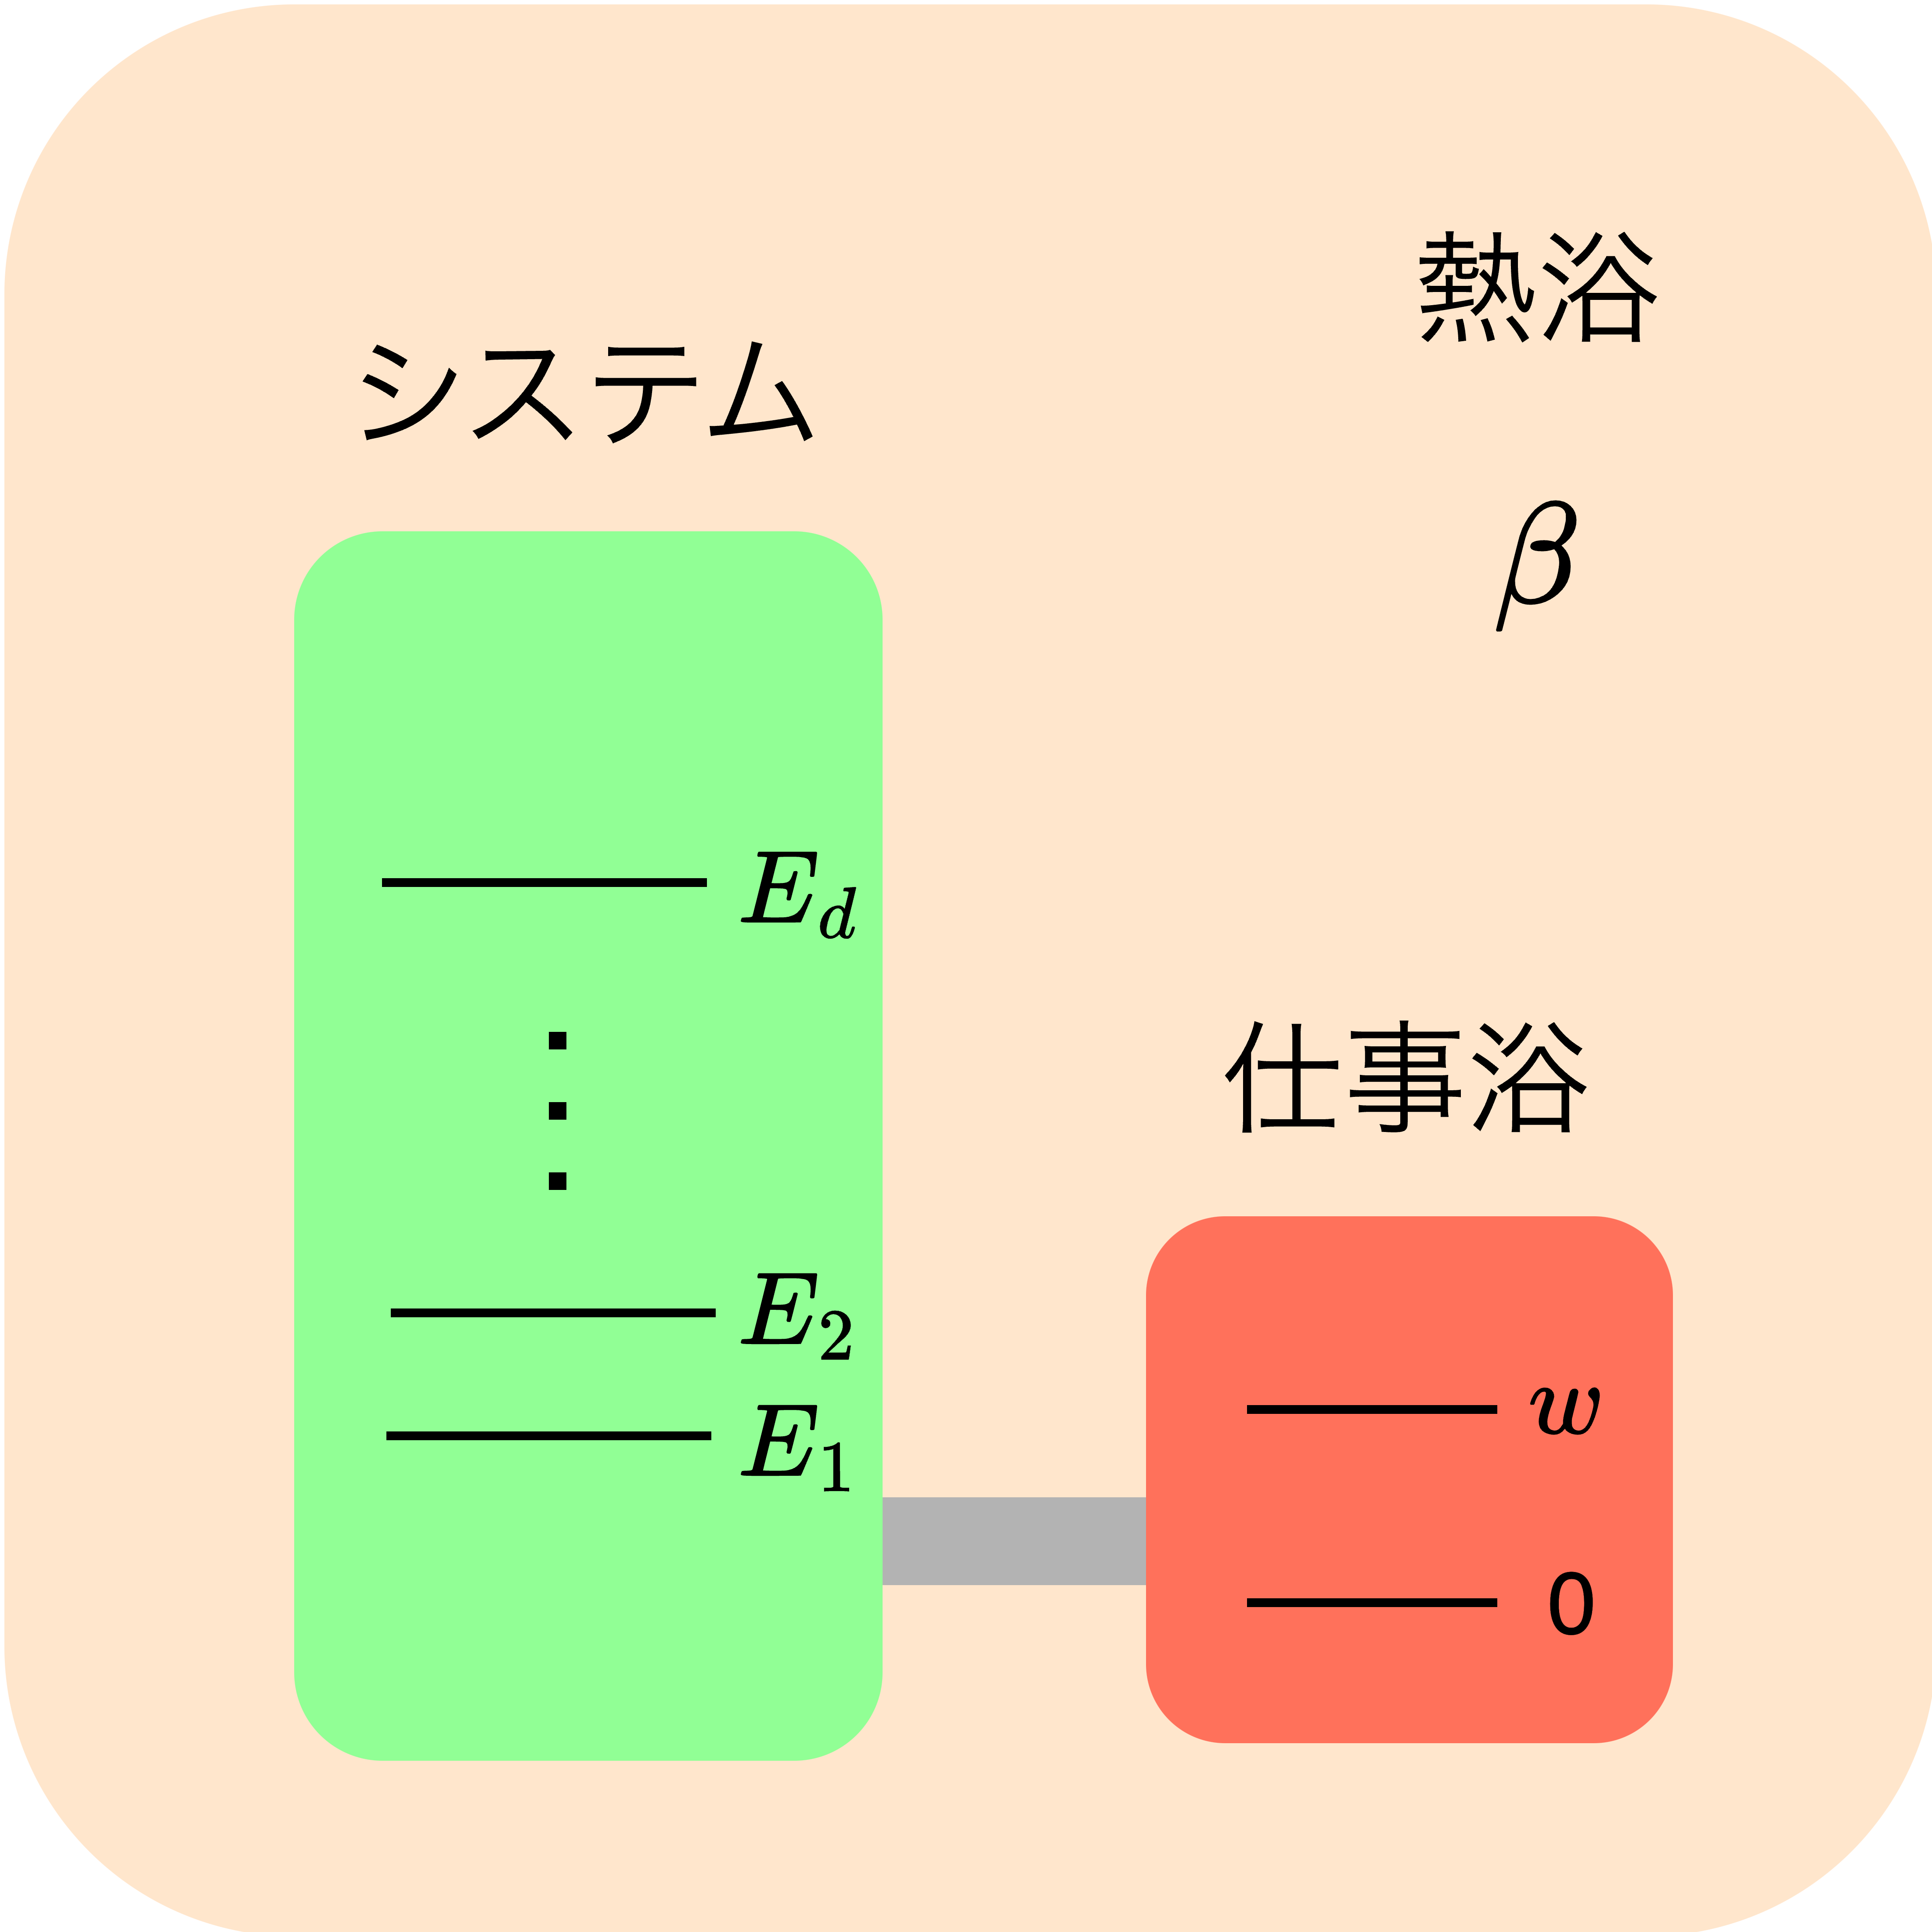
\includegraphics[keepaspectratio, scale=0.04]{images/Single-Shot_quantumthermo.drawio.png}
  \caption{Single-Shotの熱力学の概念図. 
  \cite{PhysLabResource}をかなり参考にした. 
  この図だとC系がうまく作動してHamiltonianもちゃんと切り替わったようになっているが, 以下に述べるApproximate Caseではうまく切り替わらない場合もあることに注意. }
  \label{fig:Single-Shot_quantumtherm}
\end{figure}

このとき, SC系ととW系とを合わせた系全体のGibbs状態は$\hat{\rho}_{SCW}^G\coloneqq\hat{\rho}_{\text{SC}}^G\otimes\hat{\rho}_{\text{W}}^G$となる. 

この章の残りの節では, 以上のような状況設定の中で, 始状態$\hat{\rho}_i\in\symcal{S}(\symcal{H}_{\text{SC}}\otimes\symcal{H}_{\text{W}})$を指定した終状態$\hat{\rho}_{f}$に写像するGibbs保存写像が存在するかどうか, について色々と条件を変えて議論する. 
物理状態を密度演算子, 量子系の操作をCPTP写像と考えることで, Single-Shotの物理を「ある密度演算子を欲しい密度演算子にmapするような, 特定の条件を満たすCPTP写像が存在するか」で議論できるようになった. 

% \begin{myrem}
%   このpdfでは始状態, 終状態でシステムのHamiltonianは変わらないものとする. 
%   つまり, 考えるシステムの状態遷移は, (i)Gibbs状態から非平衡状態, (ii)非平衡状態からGibbs状態, (iii)非平衡状態から別の非平衡状態, の3パターンである. 
%   しかし, 実はClock系と呼ばれる, 自律的にシステムのHamiltonianを切り替えてくれる補助系をシステムにくっつけることで, 異なるHamiltonianの間の平衡状態遷移可能性も議論することができる\cite{SagawaEntropy}. 
%   今回のpdfでは簡便のためにC系なしで考えられる, (i), (ii)に絞って議論する. 
% \end{myrem}

